\documentclass{home_assignment}
\usepackage{nccmath}
\begin{document}
    \titlePage{Energy Environment and Society Assignment}{July 29, 2021}{Dr. Jagan Nath Shrestha}
    \problem{Prepare an engineering PV based power supply working layout diagram (indicating size of PV modules/array, size of rechargeable battery/batteries, wire sizes fuses, etc.) to meet the following requirements for a remote area school:
    \begin{enumerate}
        \item Light load: 5 nos of 15 W LED lamps for 5 different rooms
        \item Computer Load: 50 desktop computers (Ten 80-Watt computers per room in 5 different rooms) 
    \end{enumerate}
    Given: \\
    System Voltage $(V)$=220 V AC, 50 Hz\\
    Solar Insolation Value=Min 4 kWh/m2/day (for 8 months); Max: 5.5 kWh/m2/day (for 4 months)\\
    Efficiency of DC to AC inverter $(\eta_i)$=90\%\\
    Operation hours $(O_H)$= 10 hours/day\\
    Assume other data as required
}
\textit{Solution:}
    \begin{fleqn}[\parindent]
        \begin{equation*}
           \begin{split}
            &\text{Total number of rooms} (R)= 5\\
            &\text{LED lamps per room} (N_B)= 1\\
            &\text{Computers per room} (N_C)= 1\\
            &\text{Power consumed per bulb} (P_B)= 15 \text{ W}\\
            &\text{Power consumed per computer} (P_C)= 80 \text{ W}\\
            &\text{Total power consumption due to LED lamps} (P_1)= R\times N_B \times P_B=5\times1\times15=75 \text{ W}\\
            &\text{Total power consumption due to computers} (P_2)= R\times N_C \times P_C=5\times10\times80=4000 \text{ W}\\
            &\text{Total power consumption} (P_T)= P_1+P_2=75+4000=4075 \text{ W}\\
            &\therefore \text{Total power consumed per room} (P_R)= \frac{P_T}{R}= \frac{4075}{5}= 815\text{ W}\\
            &\Rightarrow \text{Total current requirement through wires} (I_W)= \frac{P_R}{V} = \frac{815}{220}=3.7 \text{ A}
             \end{split}
           \end{equation*}
        \end{fleqn}
        According to the reference for wire size and current carrying capacity relation, single strand wire of size 1/18 is required for $5$ A current, which is sufficient for our requirement.
        \\
        To proceed in solving the aforementioned requirements, some assumptions are made:
        \begin{fleqn}[\parindent]
            \begin{equation*}
               \begin{split}
                &\text{Peak sun time} (S_{peak})= 4 \text{ hours}\\
                &\text{Unit battery pack} (B_0)= 12 \text{ V}\\
                &\text{Efficiency of PV module} (\eta_{PV})=20\%
                 \end{split}
               \end{equation*}
            \end{fleqn}
            We can now proceed as,
    \begin{fleqn}[\parindent]
                \begin{equation*}
                   \begin{split}
                    &\text{Total energy requirement per day} (E_R)= P_T\times O_H= 4075\times10= 40.75\text{ KWh/day}\\
                    &\text{Total energy obtained per m\textsuperscript{2} per day} (E_O)=\eta_{PV}\times \text{min\{Solar Insolation\}}=0.2\times4=0.8 \text{ KWhm\textsuperscript{-2}/day} 
                     \end{split}
                   \end{equation*}
    \end{fleqn}
    According to the problem statement, the efficiency of the DC to AC inverter is 90\%, so the actual energy required in battery is given as,
    \begin{fleqn}[\parindent]
        \begin{equation*}
           \begin{split}
            &\text{Actual energy requirement per day} (E_A)= \frac{E_R}{\eta_i}= \frac{40.75}{0.9}=45.27 \text{ KWh/day}
             \end{split}
           \end{equation*}
\end{fleqn}
If we assume that the battery size is supposed to provide full day backup, from the \textit{ELDORA VSP.72.AAA.03} PV module specifications,
\begin{fleqn}[\parindent]
    \begin{equation*}
       \begin{split}
        &\text{Peak power per panel} (P_{peak})= 300 \text{ W}\\
        &\text{Number of panels required} (N_P)= \text{?}\\
        &\text{We have the relation,}\\
        &E_A=P_{peak}\times S_{peak}\times N_P\\
        &\Rightarrow N_P=\frac{E_A}{P_{peak}\times S_{peak}}=\frac{45270}{4\times 300}=37.725\approx 38
         \end{split}
       \end{equation*}
\end{fleqn}
\begin{figure}[H]
    \centering
    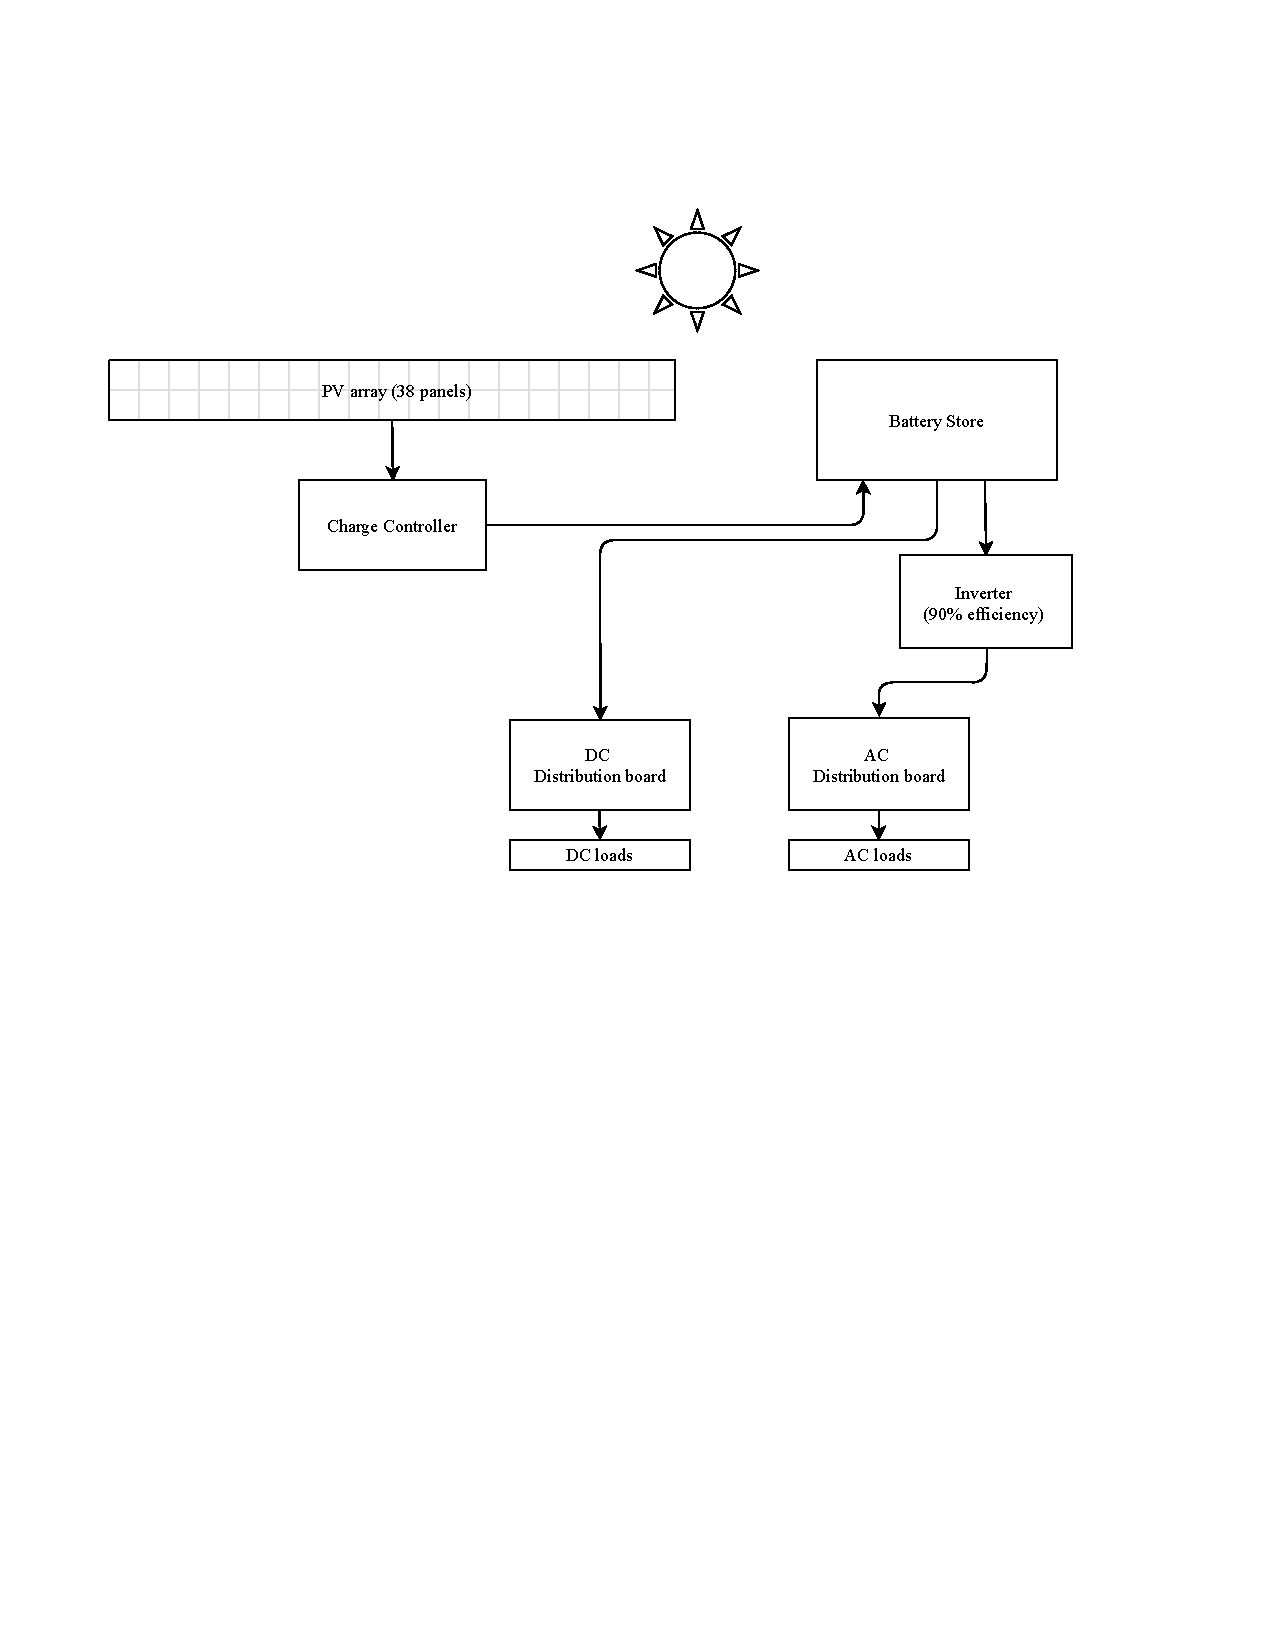
\includegraphics[width=\linewidth]{layout.pdf}
    \caption{PV based power supply layout diagram}
\end{figure}
\problem{Find out simple pay back period for Problem 1 assuming following given values:\\
Cost of PV module $(C_{PV})$= Rs. 50/Wp \\
Cost of rechargeable battery $(C_{B})$= Rs. 150/Ah of (12 V DC, DOD 80, at least 2000 Cycles)\\
Cost of sine wave inverter$(C_{I})$= Rs. 20 /Watt (24V DC/220 V AC, 50 Hz, Sine Wave) \\
Cost of diesel in remote area $(C_{RD})$= Rs. 200/litre\\
Benefits of CER US \$20/ton of CO\textsubscript{2}
}\pagebreak
\textit{Solution:}
\begin{fleqn}[\parindent]
    \begin{equation*}
       \begin{split}
        &\text{Cost per liter of diesel} (C_{D})= \text{Rs. } 108\\
        &\text{Energy generated per liter of diesel} (E_{D})=3 \text{ KWh/L}\\
        &\text{CO\textsubscript{2} emission per liter} (W_L)=2.5 \text{ Kg/L}\\
        &\text{Operational days per year} (O_Y)=280 \text{ days}       \end{split}
       \end{equation*}
\end{fleqn}
We can now calculate the diesel equivalency as,
\begin{fleqn}[\parindent]
    \begin{equation*}
       \begin{split}
        &\text{Equivalent diesel requirement per day} (V_{D})=\frac{E_R}{E_{D}} = \frac{40.75}{3}=13.6 \text{ L} \\
        &\text{Total cost of diesel per year} (C_{Diesel})= V_{D}\times C_{D}\times O_Y=13.6\times108\times280=\text{Rs. }411320\text{/year}\\
        &\text{CO\textsubscript{2} emission per year}(W_Y)=W_L\times V_{D}\times O_Y=2.5\times 13.6 \times 280=9520 \text{ Kg/year}=9.52 \text{ ton/year}\\
        &\text{Benefits due to CER of CO\textsubscript{2}} (B_{CER})=W_Y\times \$ 20=\$190.4/year\approx \text{Rs. }22630.18\text{/year}\\
        &\text{Total cost saving per year} (C_{saving})=C_{Diesel}+B_{CER}=411320+22630.18=\text{Rs. }433950.18\text{/year}\\
        &\text{Total cost expense per year} (C_{expenditure})=N_P\times C_{PV}\times P_{peak}+C_{B}\times3800+C_I\times E_R\\
        &C_{expenditure}=50\times38\times300+150\times3800+20\times4075=\text{Rs. }1221500\\
        &\text{Total payback period} (T_{payback})=\frac{C_{expenditure}}{C_{saving}}=\frac{1221500}{433950.18}=2.84\text{ years}<3 \text{ years}
         \end{split}
       \end{equation*}
\end{fleqn}
\problem{Find new answers to previous problems if number of autonomy days is considered three.}
\textit{Solution:}\\
Let us assume that battery backup for three days, charging from 0-100\% takes 6 full active usage days. So, according to \textit{6LMS200L} battery specifications,
\begin{fleqn}[\parindent]
  \begin{equation*}
     \begin{split}
      &\text{Energy capacity} (E_c)=200 \text{ Ah}\\
      &\text{Size of battery module for 3 full day backup} (S_{3days})=3772\times3 = 11316\text{ Ah}\\
      &\text{Minimum number of batteries required} (N_{battery})=\frac{S_{3days}}{E_c} =\frac{11316}{200}=56.58\approx57\\
        \end{split}
     \end{equation*}
\end{fleqn}
We have the relation,
\begin{fleqn}[\parindent]
  \begin{equation*}
     \begin{split}
      &\text{Total energy required} (E_{6days})= E_A\times9 = 45.27\times9=407.43\text{ KWh}\\
      &\text{Energy production per day} (E_{P})=\frac{E_{6days}}{6}=\frac{407.43}{6}=67.91 \text{ KWh}
        \end{split}
     \end{equation*}
\end{fleqn}
From the \textit{ELDORA VSP.72.AAA.03} PV module specifications,
\begin{fleqn}[\parindent]
    \begin{equation*}
       \begin{split}
        &\text{Peak power per panel} (P_{peak})= 300 \text{ W}\\
        &\text{Number of panels required} (N_P)= \text{?}\\
        &\text{We have the relation,}\\
        &E_{P}=P_{peak}\times S_{peak}\times N_P\\
        &\Rightarrow N_P=\frac{E_P}{P_{peak}\times S_{peak}}=\frac{67910}{4\times 300}=56.592\approx 57
         \end{split}
       \end{equation*}
      \end{fleqn}
      \problem{A BTS (Base Transceiver Station) is being planned to install at a remote area without INPS (Integrated National Power System). During active mode from 0600 hours  to 2300 hours, required current to operate the relevant equipment is 37 A and during sleep mode from 2300 hours to next day 0600 hours, required current is 10 A. The operating voltage is 48 V DC with negative grounding.
      Design PV based power system along with deep cycle battery bank with 50\% DOD (depth of discharge) for number of autonomy days considered as two. The average peak sun can be considered as 4 hours.
      }
      \textit{Solution:}
      \begin{fleqn}[\parindent]
        \begin{equation*}
           \begin{split}
            &\text{Operation time in active mode} (T_A)=17 \text{ hours}\\
            &\text{Operation time in sleep mode} (T_S)=7 \text{ hours}\\
            &\text{Current requirement for active mode} (I_A)=37 \text{ A}\\
            &\text{Current requirement for sleep mode} (I_S)=10 \text{ A}\\
            &\text{Operating voltage} (V)=48 \text{ V}\\
            &\text{Total energy in a day cycle} (E_D)= V(I_A\times T_A + I_S\times T_S)=48(37\times17+10\times7)=33.552 \text{ KWh}\\
            &\text{Total autonomy day} (T_D)=2 \text{ days}\\
            &\text{Total energy consumption} (E_T)=E_D\times T_D = 33.552\times2=67.104\text{ KWh}\\
            &\text{Depth of discharge} (DOD)=50\%\\
            &\text{Total energy capacity of battery} (E_B)=\frac{E_T}{DOD}=\frac{67.104}{0.5}=134.208\text{ KWh}
             \end{split}
           \end{equation*}
          \end{fleqn}
According to \textit{6LMS200L} battery specifications,
\begin{fleqn}[\parindent]
  \begin{equation*}
     \begin{split}
      &\text{Energy capacity} (E_c)=200 \text{ Ah}\\
      &\text{Voltage} (V_B)=12 \text{ V}\\
      &\text{Size of battery module} (S_{B})=\frac{E_B}{B_B} = \frac{134208}{12}=11184\text{ Ah}\\
      &\text{Minimum number of batteries required} (N_{battery})=\frac{S_{B}}{E_c} =\frac{11184}{200}=55.92\approx56\\
        \end{split}
     \end{equation*}
     Since $V=48$ V, and $V_B=12$ V system requires $\frac{V}{V_B}=4$ units in series and its multiple in parallel to increase the energy capacity. Here, $N_{battery}=56$ is a multiple of 4,hence no extra battery must be added to attain 48 V serial packs.
\end{fleqn}
From the \textit{ELDORA VSP.72.AAA.03} PV module specifications,
\begin{fleqn}[\parindent]
    \begin{equation*}
       \begin{split}
        &\text{Peak power per panel} (P_{peak})= 300 \text{ W}\\
        &\text{Number of panels required} (N_P)= \text{?}\\
        &\text{We have the relation,}\\
        &E_{D}=P_{peak}\times S_{peak}\times N_P\\
        &\Rightarrow N_P=\frac{E_P}{P_{peak}\times S_{peak}}=\frac{33552}{4\times 300}=27.96\approx 28
         \end{split}
       \end{equation*}
      \end{fleqn}
\end{document}